% BOF Preamble
\documentclass[cmpstyle]{ueacmpstyle}
% imports
\usepackage{fancyhdr}
\usepackage{csquotes}
\pagestyle{fancy}
\fancyhead{}
\fancyfoot{}
\lfoot{100104118, 100036248}
\rfoot{Page \thepage}
\renewcommand{\footrulewidth}{0.4pt}
% macros
\newcommand{\nt}{\textsc{NorwichTravel}}
% EOF Preamble

% BOF Document
\begin{document}
	% BOF Title & Abstract
	\title{\textsc{NorwichTravel}: developing usable software}
	\author{Jack C. Penson, Christopher A. Irvine}
	\date{\today}
	\maketitle
	\begin{abstract}
		As technology becomes more accessible and prevalent in today's society, the demand in industry for Mobile Applications to be accessible to all potential users is growing. \nt \ is an app built in React Native with a focus on ease of use. Specifically handling users who are visually impaired and might posses limited motor skills. %weak word growing% 
	\end{abstract}
	% EOF Title & Abstract
	% BOF Introduction
	\section{Introduction} \label{sec:intro}
	In this report we will explore what it means for a Mobile Application (app) to be usable and accessible to all potential users. Specifically looking into the industry standard guidelines related to Mobile Applications. Then we follow the development cycle of \nt \ as it progresses to be increasingly more user friendly and accessible. Finally we will examine techniques and methods for testing the accessibility of an app, as we perform them on \nt, to discern what improvements could be made in the future to improve \nt.
	
	\textit{Usability} is defined as ``How effectively, efficiently and satisfactorily a user can interact with a user interface''; whereas \textit{Accessibility} is defined as ``The measure of a web page's usability by persons with one or more disabilities'' \citep{usability}. The difference between the two is that accessibility is about usability for those with disabilities.
	
	In order to develop an app that is accessible we must first develop the app to be usable. Once that has been achieved the development is a balancing act between maintaining usability whilst integrating accessibility, at the same time keeping the integrity of the design.
	
		\subsection{Scenario} \label{sec:scenario}
		\nt \ will be developed using a scenario; which is a quick and easy way to define the features of a service, so that the scope of the project does not expand.
		
		\blockquote{Steve is a student at UEA and it is the end of the semester. He has just submitted his last assignment and one of his friends, Sally, suggests that they go out tonight. Sally, who is visually impaired, wants to go and get dinner in town, see a film and grab a couple of drinks with her course mates before everyone scatters for the holidays. They want to get the bus into town, but will likely need a taxi back after spending a couple of hours in the pub. Steve also needs to go back for the Christmas Holidays during the weekend, he normally has his train ticket booked up by now, but this year he hasn't. So he will need to check what trains are heading to Cambridge from Norwich. The group of friends break up to leave their bags at their respective houses and agree a time to meet in town. Knowing that the bus will take around 20 minutes to get into town, Sally needs to find out what time the bus will be at the stop so that she doesn't have to wait out in the cold for longer than she has to.}
	
	% EOF Introduction
	% BOF Usability and Accessibility Discussion
	\section{Usability and Accessibility} \label{sec:UnA}
	As we learned in Section \ref{sec:intro}, there is a three-way balancing act between design, usability and accessibility. These elements can and do complement each other in many ways, but should one take priority during the development of a system, the other two will suffer immensely. In this section we will examine the individual elements ``balancing act'' in detail, in addition to why it is important that app developers should concern themselves with such a task.
	
		\subsection{Why is Usability and Accessibility Important?} \label{sec:important} 
		The price of smartphones has drastically fallen worldwide (with the exception of the United States, where we can observe a small increase) \citep{smartphonePrice}. This means that smartphones, and the apps that can be used on them are becoming increasingly accessible. As more users can access a smartphone the percentage of users who live with some sort of disability increase \citep{ofcom}. These disabilities can range from an elderly individual with diminishing eyesight to someone who suffers from a serious affliction such as motor neuron disease. As well as accessibility increasing importance, the falling prices of smartphones also bring entirely new users into the user base. If the apps that they want to use are not usable they will quickly move on in frustration.
		
		Due to this change in the user base, developers need spend more of their resources catering for them. Services that do not devote sufficient resources to integrate accessibility and usability features, are essentially denying themselves potential users. 13 million people in the UK have some kind of disability, which is $\frac{1}{5}\textsuperscript{th}$ of the population \citep{disabledUK}. This does not only to app developers, web developers need to make their websites as usable and accessible as possible.
		
		\subsection{Industry Guidelines} \label{industry}
		With the user base changing for the web and app industries, the consensus is that Usability and Accessibility is indeed important and there should be metrics and guidelines in place to ensure that the disabled user base is looked after in the proper manner. The World Wide Web Consortium (W3C), ``an international community where Member organisations, a full-time staff and the public work together to develop web standards.'' \citep{W3Cwho}, developed a set of guidelines (including metrics) for web developers to follow. These guidelines are known as the ``\textit{W3 Accessibility Guidelines}'' \citep{w3guide}. Whilst these guidelines are principally aimed towards websites, there is a dedicated section to mobile usability and accessibility including a separate set of metrics. In addition to the guidelines, there are several services that serve to check if your website (or app in some cases) comply with the W3 Accessibility Guidelines. One such example is the WebAIM: Color Contrast Checker, seen in Figure \ref{fig:contrast-check} \citep{contrast-check}.
		
		\begin{figure}
			\centering
			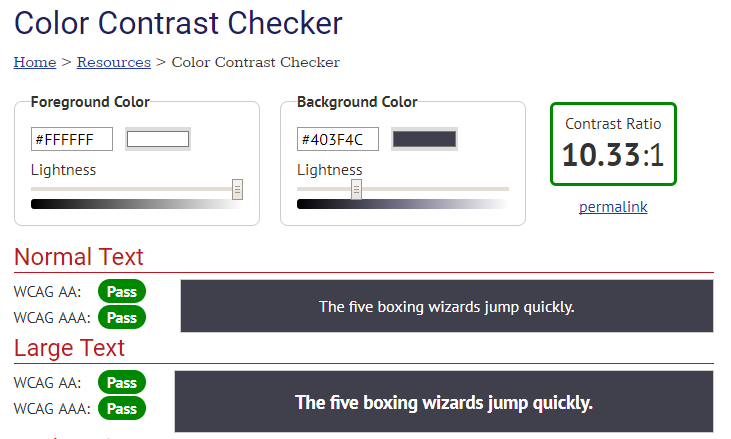
\includegraphics[height=7cm]{images/contrast-checker.png}\\
			\caption{A screenshot taken from \citep{contrast-check} displaying the results from checking the Colour Contrast on \nt. The hex codes for the two main colours of the design is entered into the ``Foreground Color'' and ``Background Color'' boxes, the results are displayed below.}\label{fig:contrast-check}
		\end{figure}
		
		\subsection{Considerations towards Developers} \label{sec:devcons}
		Usability and Accessibility is not an issue that concerns only the users of a system. The developers have to invest significant time and resources into integrating Operating System level features, such as the iOS Magic Touch, into their apps. Unfortunately, many developers underestimate the increase in complexity that accessibility brings. This can lead to projects being exceeding their budget and time limits.
		
		This is why for the development of \nt, React Native was chosen. React Native is a cross platform JavaScript library that has integrated many of the Operating System level accessibility features into itself \citep{reactAccess}. Due to this integration, we can override the default screen readers with more informative labels, or set the iOS Magic Tap to perform specific tasks, both of which will be addressed in greater detail in Section \ref{sec:nortrav}.
		
	% EOF Usability and Accessibility Discussion
	% BOF NorwichTravel overview
	\section{\nt} \label{sec:nortrav}
	As we learned in Section \ref{sec:scenario}, \nt \ was developed through the use of a Scenario. The Scenario is broken down into a list of \textit{User Stories} that is then translated into a list of functionality for the app. There are two main advantages to developing through Scenarios; it is a simple method to generate functionality, but more importantly it places the user at the centre of the app from the very start of the development cycle. See Section \ref{sec:prop-func} for a full list of proposed functionality from the Scenario.
	
	From Section \ref{sec:devcons}, we learned that \nt \ is a React Native app. Allowing for easy Cross-Platform (iOS and Android) support and rapid prototyping when used in conjunction with services such as Expo \citep{expo}. In addition to the support that React Native has for accessibility functionality (see Section \ref{sec:devcons}).
	
		\subsection{Proposed Functionality} \label{sec:prop-func}
		\nt \ is an app that provides public transport information for Norwich. The three principle forms of public transport within Norwich are Buses, Trains and Taxis. Below is the list of functionality related to information about the aforementioned public transport:
			\begin{itemize}
				\item Look up Bus Times from a Bus Stop within Norwich.
				\item Look up the next Train Times from Norwich Station.
				\item Look up the time of the next Train from Norwich to a given location.
				\item Find a list of Taxi companies that operate within Norwich. 
			\end{itemize} 
		
		\subsection{Target Audiences} \label{sec:target}
		
		\subsection{Documentation Overview} \label{sec:doc-over}
	% EOF NorwichTravel overview
	% BOF Design Discussion
	\section{Designing for Usability and Accessibility} \label{sec:design}
	
		\subsection{Conforming to Guidelines} \label{sec:conform}
		
		\subsection{Compromises Made} \label{sec:comp}
	% EOF Design Discussion
	% BOF Evaluation and Testing
	\section{Evaluating \nt} \label{sec:eval}
	
		\subsection{Prototyping} \label{sec:proto}
		
			\subsubsection{Think-Aloud Evaluation} \label{sec:think}
			
		\subsection{``Glasses'' Test} \label{sec:glasses}
		Both of the developers working of \nt \ posses diminishing eyesight. At the suggestion of the Project Supervisor, one of the principle testing methods that was employed throughout \nt's development cycle was the ``Glasses'' Test. A developer to load the app on a phone, through Expo, and remove their glasses. The phone would be positioned in such a way that it became hard to see. The developer would have to then complete a set of tasks with and without the screen reader active. Any issues that were encountered could be noted immediately by the developer. 
		
		This test proved extremely effective, due to its similarity to the Think-Aloud Evaluation. The crucial difference is that the developer does not have to convey their thoughts to an evaluator. Instead they can note down the issues they encounter in a manner that makes sense to them and then immediately act upon them. 
		
		\subsection{Industry Tools} \label{sec:industry-tools}
		
		\subsection{Results and Adjustments to \nt} \label{sec:adjust}
			
			\subsubsection{Major Issues} \label{sec:major}
			
			\subsubsection{Addressing Issues} \label{sec:address}
			
			\subsubsection{Open Issues} \label{sec:open}
	% EOF Evaluation and Testing
	% BOF Conclusion
	\section{Conclusions} \label{sec:conc}
	
		\subsection{Was \nt \ fit for purpose?} \label{sec:fit}
		
		\subsection{Was \nt \ accessible to the target user groups?} \label{sec:accessibletotarget}
	% EOF Conclusion
	
	\bibliographystyle{abbrvnat}
	\bibliography{report}
	
	\appendix
	\section{Prototypes}
	
	\section{UML Diagrams}
\end{document}

% EOF Document